%!TEX root = ../Studienarbeit.tex

\chapter{Umsetzung}

\section{Softwareentwicklung}
In diesen Abschnitt werden einige Kernkomponenten der Software detaillierter dargestellt und die Auswahl des Mikrocontrollers beschrieben.

\subsection{Auswahl der Mikrocontrollers}
Als Mikrocontroller wird das ESP32-WROOM-32E-Modul verwendet. Dies hat mehrere Gründe, welche nachfolgend zu finden sind.
Als erster Grund, welcher für die Verwendung des ESP32 spricht, ist die große Beliebtheit des Mikrocontrollers in Hobbyprojekten und daraus folgernd eine große Community die bei Problemen in der Entwicklung unterstützen kann \cites{redditESP32}{esp32Forum}. Ebenfalls ist eine gute Dokumentation der \ac{ESP-IDF} durch Kommentare im Sourcecode, sowie durch Beispielprogramme gegeben. Als weiterer Grund für die Verwendung des ESP32 spricht, die Unterstützung mehrerer Bluetooth-Stacks, welche in Kapitel \ref{section:bluetoothStacks} beschrieben sind. Als letzter Grund ist noch die Verfügbarkeit der Mikrocontroller in kompakten Hardwaremodulen, in denen alle benötigen Hauptkomponenten für den Betrieb des Mikrocontrollers enthalten sind, wie Kondensatoren, Widerständen und in manchen Modulen ebenso die benötigte Antenne für den Betrieb von Bluetooth oder \acs{WLAN} \cite[S.~14]{espressifHardwareDesignGuidelines}. Auch haben die ESP32-Module meist eine CE-Zertifizierung, wie in Kapitel \ref{section:esp32Explained} beschrieben ist und dadurch könnte das entwickelte Fernsteuerungsmodul vereinfacht für den Vertrieb zertifiziert werden. Trotz den vorhandenen Funktionsumfang und Ökosystem ist das ESP32-Modul kostengünstig und im Bereich um 5~€ zu erwerben \cite{espressifModules}.

\subsection{Auswahl des Bluetooth-Stacks}
Als Bluetooth-Stack für den ESP32 wird der Open Source \ac{BLE}-Stack Apache NimBLE verwendet. Dies hat den Hintergrund, dass die Kommunikation ausschließlich zwischen dem Fernsteuerungserweiterungsmodul und Endgeräten mittels \ac{BLE} erfolgen soll. Für diesen Einsatzzweck wird die Verwendung von Apache NimbLE empfohlen, da dieser kompakter in der Codegröße ist und weniger Speicher zur Laufzeit benötigt \cite{espidfBluetoothStack}.

\subsection{Kommunikation zwischen dem Mikrocontroller und dem Endgerät}
\label{section:communicationModuleDevice}
Für die Übermittlung der Daten zwischen dem Mikrocontroller zu einem Endgerät wird \ac{BLE} verwendet, indem die Fernsteuerungsdaten mittels \ac{HOGP} verpackt werden. \ac{BLE} wird verwendet, da es sich besser für eine mobile Anwendung eignet -- beschrieben in Kapitel \ref{section:bluetoothGenerall} --, da die Multikopterfernsteuerung und das Erweiterungsmodul mittels demselben Akku betrieben werden und dadurch die Akkulaufzeit verlängert werden kann. Als Datenformat wird \ac{HID} verwendet, da es dadurch möglich ist ohne speziell entwickelten Treibern die Daten am Endgerät auszuwerten und dadurch der Datenaustausch zwischen dem Modul und vielen Endgeräten sichergestellt werden kann \cite{microsoftHID}. In der Tabelle \ref{table:usedServicesAndCharacteristics} sind alle verwendeten \ac{BLE}-Dienste mit zugehörigen Merkmalen aufgelistet. Zusätzlich enthält das Report-Merkmal einen Konfigurationsdeskriptor, womit sich Endgeräte zu den Report abonnieren können, womit bei Änderung der Daten automatisch die Endgeräte mit den neuen Daten versorgt werden. 

\begin{longtable}[c]{|l|l|}
    \caption{Liste der verfügbaren Geräteinformationsmerkmale}
    \label{table:usedServicesAndCharacteristics}\\
    \hline
    \textbf{\ac{BLE}-Dienst} & \textbf{Merkmale}\\
    \hline
    \hline
    \endfirsthead

    \hline
    \textbf{\ac{BLE}-Dienst} & \textbf{Merkmale}\\
    \hline
    \hline
    \endhead

    \hline
    \multicolumn{2}{|r|}{Weitere \ac{BLE}-Dienste auf der nächsten Seite}\\
    \hline
    \endfoot

    \hline
    \endlastfoot
    
    \multirow{4}{*}{Geräteinformationsdienst} & Herstellername\\
    \cline{2-2}
     & Modellnummer\\
     \cline{2-2}
     & Firmwareversion\\
     \cline{2-2}
     & Softwareversion\\
    \hline
    \multirow{1}{*}{Batteriedienst} & Akkustand\\
    \hline
    \multirow{4}{*}{\ac{HID}-Dienst} & Report-Map\\
    \cline{2-2}
     & \ac{HID} Information\\
     \cline{2-2}
     & \ac{HID} Control Point\\
     \cline{2-2}
     & Report definiert als Eingabe\\
\end{longtable}

Der finale Report Map Deskriptor des Erweiterungsmoduls ist konfiguriert, dass die übertragenden \ac{BLE}-Daten Gamepaddaten enthalten. Als Daten werden acht analoge und acht digitale Kanaldaten übertragen, welche den aktuellen absoluten Wert darstellen. Die analogen Kanäle haben dabei eine Größe von 16~Bit und haben einen Wertebereich von 0 bis 2047. In den analogen Kanälen werden mittels vier Kanälen die zwei Steuerknüppelpositionen übertragen. Mittels den restlichen vier Kanälen werden die Stellung von Kippschaltern mit drei Positionen übertragen. Die digitalen Kanäle haben eine Größe von 1~Bit und können den Wert 0 oder 1 annehmen. Diese Kanäle werden für Knöpfe mit 2 Stellungen verwendet. In Quellcode \ref{lst:reportDescriptorModule} ist der Report Deskriptor zu sehen.

Zusätzlich zur Information im Report Map Deskriptor, dass das Erweiterungsmodul als Gamepad agiert, wird im Advertising-Paket diese optionale Information ebenso bereitgestellt. Dadurch erscheint unter einigen Betriebssystemen während der Kopplung des Erweiterungsmoduls schon ein Gamepadsymbol, um den Benutzer zu zeigen, dass es sich um ein Gampad handelt, was gekoppelt wird.

\begin{lstlisting}[caption=Report Map Deskriptor des Erweiterungsmoduls, label={lst:reportDescriptorModule}, style=generalStyle]
    0x05, 0x01,        // Usage Page (Generic Desktop Ctrls)
    0x09, 0x05,        // Usage (Game Pad)
    0xA1, 0x01,        // Collection (Application)
    0x85, 0x01,        // Report Id (1)
    0xA1, 0x00,        //   Collection (Physical)
    0x05, 0x01,        //     Usage Page (Generic Desktop Ctrls)
    0x09, 0x30,        //     Usage (X)
    0x09, 0x31,        //     Usage (Y)
    0x09, 0x32,        //     Usage (Z)
    0x09, 0x33,        //     Usage (Rx)
    0x09, 0x35,        //     Usage (Rz)
    0x09, 0x34,        //     Usage (Ry)
    0x09, 0x36,        //     Usage (Slider)
    0x09, 0x36,        //     Usage (Slider)
    0x15, 0x00,        //     Logical Minimum (0)
    0x26, 0xFF, 0x07,  //     Logical Maximum (2047)
    0x75, 0x10,        //     Report Size (16)
    0x95, 0x08,        //     Report Count (8)
    0x81, 0x02,        //     Input (Absolute)
    0x05, 0x09,        //     Usage Page (Button)
    0x19, 0x01,        //     Usage Minimum (0x01)
    0x29, 0x08,        //     Usage Maximum (0x08)
    0x15, 0x00,        //     Logical Minimum (0)
    0x25, 0x01,        //     Logical Maximum (1)
    0x95, 0x08,        //     Report Count (8)
    0x75, 0x01,        //     Report Size (1)
    0x81, 0x02,        //     Input (Absolute)
    0xC0,              //   End Collection
    0xC0,              // End Collection
\end{lstlisting}

Ebenso sind alle Sollanforderungen durch Apple während der Implementierung beachtet worden, damit keine Komplikationen für Apple Geräte entstehen sollten. Zusätzliche nicht dokumentierte Anforderungen waren dabei, dass das Erweiterungsmodul das Auflösen von \ac{RPA} unterstützt, da sonst kein Verbindungsaufbau zum Datenaustausch zwischen Apple Geräten stattfindet. Eine weitere nicht dokumentierte Anforderung für Applegeräte ist, dass die Datenübertragung zwischen dem Erweiterungsmodul und dem Applegeräte verschlüsselt stattfinden muss, wenn es sich um \ac{HID}-Daten handelt. Dafür werden im ersten Schritt die Geräte gekoppelt, welches durch verschiedene Verfahren erfolgen kann. Für das Erweiterungsmodul findet die Kopplung durch das Anzeigen eines Pins auf beiden Geräten statt und das darauffolgende Bestätigen des Pins von beiden Parteien. Im darauffolgenden Schritt erfolgt das Bonding, womit die übertragenden Daten der Kopplung gespeichert werden, um bei einem erneuten Verbindungsaufbau nicht erneut eine Kopplung durchzuführen \cite{kyneticsBondingPairng}.

Für die Darstellung von Statushinweisen auf dem integrierten Display des Erweiterungsmoduls, werden alle \ac{GAP}-Events überwacht. Dadurch wird der Pin während der Kopplung dargestellt und der aktuelle Verbindungsstatus mit einem Endgerät angezeigt. Auch wird mittels eines \ac{GAP}-Events eine Anfrage von Endgeräten gestellt, um sich an einem \ac{BLE}-Merkmal zu abonnieren. Zuletzt wird das \ac{GAP}-Event, welches während dem Verbindungsaufbau auftritt verwendet, um eine Anfrage zur Gegenpartei zu schicken, damit die Verbindungsparameter angepasst werden. Durch angepasste Verbindungsparameter kann ein gestellt werden wie oft \ac{BLE}-Pakete versendet werden, wodurch die Übertragungsrate steigt.

\subsection{Kommunikationsprotokoll zwischen der Multikopterfernsteuerungen und dem Mikrocontroller}
Als Kommunikationsprotokoll zwischen der Multikopterfernsteuerung und des Mikrocontroller wird CRSF verwendet. Dies hat den Hintergrund, dass wie in Kapitel \ref{section:communicationsProtocollsRemote} das CRSF-Protokoll die höchste Übertragungsrate hat und dabei die geringste Menge an nicht verwendeten Daten versendet, da das Protokoll leicht durch die Geräteadressen und Datentypenidentifikatoren gefiltert werden kann.

Da CRSF die Daten mittels einer \ac{UART}-Verbindung übertragt, findet das Auslesen der CRSF-Daten mittels dem Mikrocontroller durch einen sogenannten Treiber statt. Durch den \ac{UART}-Treiber werden vorhandene \ac{UART}-Interrupt abstrahiert und durch eine \ac{API} bereitgestellt, wodurch die Kommunikation mittels \ac{UART} vereinfacht wird \cite{espUARTDriver}. Die \ac{UART}-Interrupt sind definiert, das empfange Daten erst verarbeitet werden, wenn entweder der interne \ac{UART}-Buffer voll ist oder ein definierter Timeout zwischen empfangenen Bytes entsteht.

Die Auswertung der empfangenen Daten ist in zwei Teile gegliedert. Im ersten Teil findet eine Überprüfung der Geräteadresse (muss 0xEE sein), der Länge der übermittelten Daten und des übermittelten Datentyps statt (muss 0x16 sein). Wenn all diese Werte stimmen findet die Überprüfung der \ac{CRC}-Prüfsumme statt, um festzustellen, ob alle Kanaldaten gültig sind. Im zweiten Teil, werden alle Kanaldaten zunächst ausgelesen und darauf im Wertebereich angepasst, damit der vollständige Wertebereich des \ac{HID}-Reports verwendet wird. Dafür werden die analogen Kanaldaten auf einen Wertebereich von 0 bis 2047 erweitert und digitale Kanaldaten wie zum Beispiel bei Knöpfen bis zu einem Wert von 992 als logisch 0 und ab einen Wert von 993 als logisch 1 gewertet. Nach Anpassung des Wertebereichs werden die Daten in einer globalen Datenstruktur abgelegt, welche in Quellcode \ref{lst:channelDataStruct} zu sehen ist. Falls dabei eine Änderung zwischen alten und aktuellen Wert festgestellt wird, wird veranlasst, dass die Daten per \ac{BLE} an das Endgerät versendet werden. Anzumerken ist, dass wenn es ein Problem während der Auswertung stattfindet, dass komplette Paket verworfen wird und auf ein neues Paket gewartet wird.

\begin{lstlisting}[caption=C-Strukuraufbau der aufbereiteten Kanaldaten, label={lst:channelDataStruct}, style=generalStyle]
    typedef struct ChannelDataStruct{
        uint16_t roll;        //roll = x
        uint16_t pitch;       //pitch = y
        uint16_t aux3;        //aux3 = z
        uint16_t yaw;         //yaw = rx
        uint16_t aux1;        //aux1 = rz
        uint16_t throttle;    //throttle = ry
        uint16_t aux4;        //aux4 = slide
        uint16_t aux2;        //aux2 = slide
        uint8_t buttons;      //buttons = aux12(b8) .. aux5(b1)
    } ChannelDataStruct;
\end{lstlisting}

\subsection{Statusausgabe des Mikrocontrollers mittels eines \acs{OLED}-Displays}
Wie in den Anforderungen in Kapitel \ref{section:softwareRequirement} und in Kapitel \ref{section:communicationModuleDevice} beschrieben, wird ein \acs{OLED}-Display verwendet, um Statusinformationen darzustellen. Dabei hat das Display eine Displaydiagonale von 0,91~Zoll, eine Auflösung von 128 zu 32~Pixeln und dem SSD1306~Displaycontroller. Die Datenübertragung zwischen dem ESP32 und dem SSD1306 erfolgt mittels \ac{I2C}. Die Ansteuerung von einzelnen Pixeln des Displays findet durch die Auswahl von Seiten und Segmenten statt. Das Display besteht aus vier Seiten mit jeweils 128 Segmenten die eine Größe von 8~Bit haben. In Abbildung \ref{fig:ssd1306PixelControl} ist zu sehen, wie ein übermittelter Datenstream auf die Seiten und die Segmente des Displays zur Darstellung übertragen wird.

\begin{figure}[h]
    \centering
    \includegraphics[width=.7\textwidth]{ssd1306}
    \caption{Verarbeitung eines Datenstreams für die Darstellung auf dem Erweiterungsmoduldisplay; abgewandelt von \cite[S.~37]{ssd1306}}
    \label{fig:ssd1306PixelControl}
\end{figure}

Zur Darstellung von Text am Display erfolgt mittels einer Bitmap-Schriftart, da die Art von Schriftarten für eine gute Lesbarkeit auf dem kleinen Display optimiert werden kann. Alle Zeichen der Schriftart werden dafür in einem zweidimensionalen Array abgelegt und weisen eine Höhe von 14 und eine Breite von 9 Pixeln auf. Zu Umwandlung von Zeichenketten in Glyphen sind zusätzliche Hilfsfunktionen implementiert. Die Darstellung von Inhalt auf dem Display erfolgt in zwei Schritten. Im ersten Schritt werden alle Pixelinformationen in einen lokalen Buffer des ESP32 zwischen gespeichert. Der Buffer hat eine Größe von 492~Byte, wo jedes Bit ein Pixel des Displays repräsentiert. Im zweiten Schritt wird der lokale Puffer mittels \ac{I2C} an das Display übertragen und dargestellt. Die Aufteilung in zwei Schritte hat den Vorteil, dass dem ESP32 immer der aktuelle Zustand des Displays bekannt ist und dass das Anzeigen von Elementen am Display einfacher ist, wenn immer der komplette Inhalt des Displays ausgetauscht wird, statt einige Regionen.

\subsection{Kombination aller Softwarekomponenten}
Die Software der Studienarbeit ist in der Programmiersprache C geschrieben, da eine Vielzahl an Bibliotheken sowie Beispielprogramme in C geschrieben sind \cite{espressifIDF}, wodurch die Integration von eigenem Code einfacher erfolgen kann. Zur Verwaltung von Threads auf dem Mikrocontroller wird FreeRTOS als Echtzeitkernel verwendet. Die finale Software des Mikrocontroller besteht aus fünf Komponenten. Die erste Komponente, welche in einen FreeRTOS-Task läuft, ist die Software welche sich komplett um die \ac{BLE}-Kommunikation und dem \ac{BLE}-Verbindungsaufbau kümmert. Die zweite Komponente, welche ebenso in einen FreeRTOS-Task läuft, kümmert sich um das einlesen und verarbeiten von CRSF-Daten, welche von der Multikopterfernsteuerung verschickt werden. Die dritte Komponente, welche als FreeRTOS Software Timer integriert ist, kümmert sich um die Bestimmung des aktuellen Akkustands. Hierfür wird mittels eines integrierten \ac{ADC} des ESP32 die aktuelle Spannung des Multikopterfernsteuerungsakkus bestimmt und in einen Prozentwert zwischen 0 und 100 umgewandelt, damit der Akkustand mittels \ac{BLE} an das Endgerät weitergeschickt wird. Die nächste Komponente der ESP32-Software ist für das Abfangen von Tasteneingaben zuständig. Das Erkennen von Tasteneingaben erfolgt dabei mittels FreeRTOS-Interrupts und die Weitergabe an die parallel laufenden Task mittels FreeRTOS-Queues. Die letzte Softwarekomponente des ESP32, ist für die Steuerung des Displays vorhanden. Da Anzeigeänderungen am Display nur selten erfolgen und schnell abgearbeitet werden, werden die Displayhilfsfunktionen innerhalb der zwei vorhandenen Tasks ausgeführt. Da der ESP32-Mikrocontroller über zwei Kerne verfügt, werden beide vorhandenen Tasks jeweils fest auf einen Kern zugewiesen, um das Blockieren zwischen den einzelnen Softwarekomponenten zu verringern.

Für den Datenaustausch zwischen dem CRSF-Task, welche die Daten der Fernsteuerung verarbeitet, und dem \ac{BLE}-Task, welcher die Daten an das Endgerät weiterschickt, werden globale Variablen zur Speicherung der Multikopterfernsteuerungsdaten verwendet. Zur Mitteilung, wenn neue Daten von der Fernsteuerung ausgewertet wurden, wird zwei bereits vorhandene Funktionen verwendet. Zum einen die Funktion \textit{ble\_hs\_mbuf\_from\_flat}. Mit dieser Funktion werden die Fernsteuerungsdaten in den internen \ac{BLE}-Buffer geschrieben. Zum anderen die Funktion \textit{ble\_gattc\_notify\_custom}, womit die Daten durch den \ac{BLE}-Task automatisch an das Endgerät versendet werden.

\subsection{Weiterführende Informationen}
Für weitere Details ist der komplette Sourcecode öffentlich unter folgenden Link zu finden:\\ \url{https://github.com/SimLinkModule/ModuleSoftware}

\section{Platinenentwurf}
Damit der vorhandene Testaufbau auf Steckbrettern kompakt, mobil und benutzerfreundlich verwendet werden kann, sind alle benötigten Elektronikkomponenten in drei Platinen integriert, welche in Abbildung \ref{fig:pcbs} zu sehen sind. Durch die Aufteilung der Elektronikkomponenten auf drei Platinen ist es möglich während der Gehäuseerstellung eine größtmögliche Flexibilität zu haben. \textit{Platine 1} dient zur Verbindung zwischen Multikopterfernsteuerung und dem ESP32. \textit{Platine 2} ist die Hauptplatine, welche die Spannungsregulierung, den ESP32-Mikrocontroller und Logik für Beschreiben des ESP32. \textit{Platine 3} enthält alle Eingabe- und Ausgabeelemente für Benutzerinteraktionen.

\begin{figure}[h]
    \centering
    \includegraphics[width=.7\textwidth]{pcbs}
    \caption{Platinen des Erweiterungsmoduls}
    \label{fig:pcbs}
\end{figure}

\subsection{Teilschaltungen}
Nachfolgend sind einige Bestandteile der Schaltungen der Platinen genauer erklärt.

\subsubsection{Spannungsregulierung}
Die Schaltung des Erweiterungsmoduls benötigt eine Spannungsregulierung, da der ESP32-Mikrocontroller mit 3,3~V betrieben wird. Die verfügbaren Spannungen durch die Mulikopterfernsteuerung liegen bei einem konstanten Wert zwischen 6~V und 12~V. Ebenso ist es möglich die Schaltung mittels der integrierten Programmierbuchse zu betreiben, bei dem die Spannung 3~V beziehungsweise 5~V sein. Zur Spannungsregulierung wird ein \ac{LDO} \ac{IC} verwendet, welcher eine Spannung höher als 3,3~V auf eine konstante Spannung von 3,3~V regelt. Zu sehen ist die benötigte Schaltung in Abbildung \ref{fig:spannungsRegulierung}. Zusätzlich enthält die Schaltung im geregelten Spannungskreis eine \acs{LED}, womit hingewiesen wird, ob eine Stromzufuhr zum ESP32-Mikrocontroller vorhanden ist.

\begin{figure}[h]
    \centering
    \includegraphics[width=.4\textwidth]{spannungsRegulierung}
    \caption{Spannungsregulierung des Erweiterungsmoduls}
    \label{fig:spannungsRegulierung}
\end{figure}

\subsubsection{ESP32 Programmierlogik}
Die Programmierung des ESP32-Mikrocontroller findet mittels einer seriellen Verbindung zum ESP32 statt. Da viele Rechner keine serielle Buchse mehr enthalten, wird zur Programmierung des ESP32 eine USB-zu-Seriell-Programmierplatine verwendet. Alternativ könnte ein USB-zu-Seriell-Converter \ac{IC} direkt auf der finalen Platine hinzugefügt werden, was jedoch für die einmalige Programmierung unnötige Kosten und verschwendeten Platz auf der Platine mit sich führen würde. Die verfügbare ESP32-Programmiersoftware für Desktoprechner verfügt über die Option automatisch den ESP32-Mikrocontroller in einen Programmiermodus zu starten. Dafür verwendet die Software zwei Statusleitungen einer seriellen Verbindung. Zum einen die \textit{Data Terminal Ready}-Leitung und zum anderen die \textit{Request To Send}-Leitung. Zusätzlich zu den zwei Statusleitungen werden noch zwei Transistoren benötigt -- zu sehen in Abbildung \ref{fig:autoFlash} --, um die Kontakte \textit{EN} und \textit{Boot} des ESP32 zu setzen. Wenn am Kontakt \textit{EN} ein Pegel von 3,3~V anliegt, ist der ESP32 lauffähig und bei einem Pegel von 0~V findet keine Ausführung auf dem ESP32 statt. Mit dem Kontakt \textit{Boot} kann während des Starts des ESP32 festgelegt werden, ob der ESP32 in den normalen Ausführungsmodus (Pegel 3,3~V) startet oder in den Programmiermodus (Pegel 0,0~V). Der maximale Spannungspegel der seriellen Verbindung muss 3,3~V betragen.

\begin{figure}[h]
    \centering
    \includegraphics[width=.4\textwidth]{autoFlash}
    \caption{ESP32 Programmierlogik}
    \label{fig:autoFlash}
\end{figure}

\subsubsection{Tastenentprellung}
Die Tasten der Platine sind mittels internen Pull-Up Widerständen -- 45K Ohm -- mit dem ESP32-Mikrocontroller verbunden. Durch den Pull-Up Widerstand liegt bei nicht Bestätigung des Tasters eine Spannung von 3,3~V am Kontakt des ESP32 an. Wenn nun ein Taster betätigt wird, wird die Spannung am Kontakt auf 0~V gezogen, wobei zu Beginn es zu Sprüngen zwischen 0~V und 3,3~V kommt, bis sich Schlussendlich die Spannung bei 0~V einregelt. Um dieses Verhalten zu verhindern und der Taster immer eindeutige Werte bereitstellt muss der Knopf entprellt werden. Eine Möglichkeit ist, mittels eines parallel platzierten Kondensators zu kompensieren \cite{debounceButton}. In Abbildung \ref{fig:buttonDebounce} ist der Schaltungsaufbau zum entprellen der Taster zu sehen. Jedoch ist in der Abbildung der Pull-Up Widerstand nicht zu sehen, da er fester Bestandteil des ESP32 ist und daher nicht im Schaltplan mit eingezeichnet werden muss.

\begin{figure}[h]
    \centering
    \includegraphics[width=.4\textwidth]{buttonDebounce}
    \caption{Tastenentprellung durch Hardware}
    \label{fig:buttonDebounce}
\end{figure}

Beachtet werden muss, dass der Taster zum manuellen Starten des ESP32 im Programmiermodus nicht durch diese Hardwareschaltung entprellt werden darf, da beim Verbinden des Erweiterungsmoduls mit Strom der \textit{Boot}-Pin auf 0~V liegt, bis der Kondensator aufgeladen ist. Das hat zur Folge, dass der ESP32 beim ersten Start nach der Verbindung mit Strom immer in den Programmiermodus landet und im Nachhinein neu gestartet werden, müsste ohne die Stromverbindung zu trennen.

\subsubsection{\acf{ESD}-Schutz}
Um zu vermeiden, dass durch elektrostatische Aufladung des Körpers das Erweiterungsmodul beschädigt wird, wenn die Buchse zur Fernsteuerung angefasst wird, müssen diese Kontakte zusätzlich geschützt werden. Dies erfolgt durch die Zener-Dioden, welche in Gegenrichtung auf 0~V gelegt werden und in Abbildung \ref{fig:esdProtection} zu sehen sind. Die Zener-Dioden sind so dimensioniert, dass ab einer Spannung die größer als 12~V an der Spannungsversorgung oder größer als 3,3~V an der Datenleitung ist durch die Zenerdiode auf 0~V geleitet wird.

\begin{figure}[h]
    \centering
    \includegraphics[width=.4\textwidth]{esdProtection}
    \caption{\ac{ESD}-Schutzschaltung}
    \label{fig:esdProtection}
\end{figure}

\subsection{Referenzschaltungen}
Damit Fehler während des Schaltungsentwurfs vermieden werden und die Anzahl von Prototypenversionen minimiert werden kann, sind die Schaltungen der Platinen auf Referenzdesigns bereits vorhandenen Platinen aufgebaut, welch in nachfolgender List stehen.
\begin{itemize}
    \item \acs{OLED}-Schaltplan von ShenZhen QDtech Co. LTD; Stand: 24.~Juli~2019
    \item ESP32\_DevKitc\_V4-Schaltplan von Espressif Systems (Shanghai Co., Ltd.); Stand: 7.~Juni~2018
    \item Produktspezifikation des OEL Display Module von Allvision technology Inc.; Version: B
\end{itemize}

\subsection{Weiterführende Informationen}
Der Entwurf der Platinen erfolgte in der kostenlosen und Open Source Software KiCad statt \cite{aboutkicad}. Die Produktion und die Bestückung des Großteils aller Elektronikkomponenten fand durch das Unternehmen \href{https://jlcpcb.com/}{JLCPCB} statt.

Die vollständigen Schaltpläne aller Platinen sind im Anhang in Abbildung \ref{fig:mainPCB}, \ref{fig:ioPCB} und  \ref{fig:connectorPCB} zu finden und weitere Details aller Platinenentwürfe sind öffentlich unter folgenden Link zu finden:\\ \url{https://github.com/SimLinkModule/PCB}

\section{Gehäuseerstellung}
Damit die entworfenen Platinen im Modulschacht der Fernsteuerung fest und kompakt befestigt werden können, gibt es ein entworfenes Kunststoffgehäuse für Modulschächte des Typs Lite, welches im Anhang in Abbildung als Explosionszeichnung \ref{fig:shellPartsExplosion} zu sehen ist. Das Hauptaugenmerk in der Entwurfsphase lag dabei darin, dass möglichst wenig Stützstrukturen für einen Druck mittels eines \ac{FDM}-3D-Druckers benötigt werden. Dies hat den Hintergrund, dass die Oberflächen, an denen Stützstrukturen anliegen, häufig größere Nachbearbeitung benötigt und auch die Druckqualität an diesen Stellen schlechter ist. Um ohne Stützstrukturen auszukommen müssen Überhänge im Modell vermieden werden, da der 3D-Drucker nur ausgehend von der Druckgrundplatte aus drucken kann. Falls Überhänge benötigt werden muss entweder das Modell in mehrere Teilmodelle aufgeteilt werden, welche dann einzeln ohne Stützstrukturen gedruckt werden können (Zu sehen in Abbildung \ref{fig:overhangCut}). Anderseits können Überhänge gedruckt werden, wenn das Modell integrierte Stützstrukturen hat, welche einen kleineren Winkel als 45 Grad zur Druckgrundplatte aufweisen (Zu sehen in Abbildung \ref{fig:overhangStruct}).

\begin{figure}[h]
    \centering
    \includegraphics[width=.8\textwidth]{overhangCut}
    \caption{Modell mit Überhängen für den 3D-Druck vorbereiten}
    \label{fig:overhangCut}
\end{figure}

\begin{figure}[h]
    \centering
    \includegraphics[width=.5\textwidth]{overhangStruct}
    \caption{Modell mit Überhängen für den 3D-Druck vorbereiten}
    \label{fig:overhangStruct}
\end{figure}

Zur Befestigung der Platinen und des Gehäusedeckels mit dem Gehäuse, sind Löcher für Gewindeeinsätze an allen benötigten Stellen integriert. Dadurch hat das Gehäuse Gewindegänge aus Messing, wodurch alle Schrauben ohne Einschränkungen öfter rein und herausgedreht werden können, da nicht auf Gewindegang aus Kunststoff geachtet werden muss, welcher leicht beim Festschrauben und Überdrehen von Schrauben beschädigt werden könnte. Zu sehen sind alle Messinggewindeeinsätze des Gehäuses in Abbildung \ref{fig:pcbMounts}.

\begin{figure}[h]
    \centering
    \includegraphics[width=.4\textwidth]{pcbMounts}
    \caption{Messing Gewindeeinsätze zur Befestigung der einzelnen Modulkomponenten}
    \label{fig:pcbMounts}
\end{figure}

Sodass der Deckel des Gehäuses mit den Schienen für den Modulschacht und den Befestigungen der Platinen ohne Stützstrukturen gedruckt werden kann, ist der Deckel in zwei Modelle aufgeteilt. Beide Modell sollten für höhere Stabilität nach dem Druck mittels Kleber verbunden werden. Zur Befestigung der Platine für die Verbindung zwischen Multikopterfernsteuerung und dem Mikrocontroller gibt es weitere gedruckte Halterungen. Dies ist nötig, da die Platine sehr nah an der Gehäuseaußenkante liegen muss, um eine Verbindung mit dem Stecker der Fernsteuerung herstellen zu können. Zu sehen sind alle eingebauten Platinen in Abbildung \ref{fig:moduleAssembly}, sowie die Position der Modulbuchse zur Verbindung mit der Mulikopterfernsteuerung.

\begin{figure}[h]
    \centering
    \includegraphics[width=1\textwidth]{moduleAssembly}
    \caption{Eingebaute Platinen im Gehäuse}
    \label{fig:moduleAssembly}
\end{figure}

Zum Schutz der Taster und um die Tastendruckfläche zu vergrößern, sind Knöpfe im Gehäuse integriert. Zu beachten ist, dass nur Knöpfe im Gehäuse für die Tasten auf der Platine mit \acs{OLED}-Display enthalten sind, da diese nur vom Benutzer des Erweiterungsmoduls, während dem normalen Betrieb betätigt werden sollen. Die integrierten Knöpfe des Gehäuses und das Gehäuse selbst sind dabei ein Bauteil und benötigen daher keinen Zusammenbau nach dem Druck. Da durch die Integration in das Gehäuse der Knopf bewegbar gemacht werden muss, gibt es eine Verjüngung im Verbindungsstück zwischen Knopf und Gehäuse. Zu sehen ist der Knopf mit Verbindungsstück zum Gehäuse in Abbildung \ref{fig:buttonShell}. Wie ebenso im Querschnitt des Knopfes zu sehen ist, enthält der Knopf einen konischen Zylinder. Dieser ist vorhanden zum einen vorhanden, um die Tastendruckfläche des kleinen Platinentasters zu vergrößern. Zum anderen, um die Lücke zwischen Platine und Gehäuse zu überbrücken, da die Platine nicht direkt am Gehäuse befestigt werden kann.

\begin{figure}[h]
    \centering
    \includegraphics[width=0.6\textwidth]{buttonShell}
    \caption{Tasterschutz für Taster der Platine}
    \label{fig:buttonShell}
\end{figure}

\subsection{Weiterführende Informationen}
In Abbildung \ref{fig:moduleComplete} ist das fertig zusammengebaute Erweiterungsmodul zu sehen. Der Entwurf fand dabei in der kostenlosen und Open Source Software OpenSCAD statt \cite{aboutOpenScad}. Alle Modelle sind öffentlich unter \url{https://github.com/SimLinkModule/Shell} auffindbar.

\begin{figure}[h]
    \centering
    \includegraphics[width=0.3\textwidth]{moduleComplete}
    \caption{Zusammengebautes Erweiterungsmodul}
    \label{fig:moduleComplete}
\end{figure}